\section{Theory}\label{sec:theory}

This section discusses the theory behind the models used in the study, there are a few base models (section \ref{sec:theory:linreg}, and \ref{sec:theory:lstm}) based on the interpretation of the papers hand picked for this study

\subsection{Linear regression}\label{sec:theory:linreg}

The regression model will be for the sake of convenience be expressed as the following expression
$$
\vec{F}(\mathbf{A})\vec{\beta}=\vec{y}+\vec{\varepsilon}
$$

Where $\vec{F}$\marginpar{The $\vec{F}$ is not important, just that your data is shaped by a function.}\todo{Remove} is a vector function with following domain $\vec{F}:\mathbb{R}^{m\times n}\to \mathbb{R}^{m\times p}$ where $m,n,p\in \mathbb{N}$, $\mathbf{A}$ is the data in matrix form with dimensions $\mathbb{R}^{m\times n}$, $\vec{\beta}$ is the regression terms, $\vec{y}$ is the target (TJM10 or TJM20), and $\vec{\varepsilon}$ is the residual error.

This basic model to express the linearity of the components to soil temperature. This will function as the base model for regression models. 

\subsection[Plauborg Regression]{Plauborg linear regression model with Fourier terms}\label{sec:theory:pluborg}

An improvemnt over an time independent linear regression model would be a time dependent linear regression model that takes not only current time into account of the calculations but also previus messurments. It is current knowlage that soil temperatures depends on previous temperatures and metrological phenomenons. In the paper \citetitle{plauborg_simple_2002} the author chose to extend the features from only air temperature at current time to include also previus days of year and the air temperature from those days. This means the following F function that \citeauthor{plauborg_simple_2002} used would be 
$$
\vec{F} := [air_t , air_{t-1}, air_{t-2}, air_{t-3}, \sin(\omega t) , \cos(\omega t), \sin(2*\omega t), \cos(2*\omega t)]^T
$$

Where $air_t$ is the air temperature at time $t$ expressed in day of the year (0-365), $\omega$ is the angular frequency in radians per hour or radians per day, depending on the time unit. The sine/cosine elements in the F function represent the variations through the day by fitting $\vec{\beta}$ to the yearly variation. To adapt the authors model to an hourly time unit would be to either
\begin{enumerate}
	\item Extend the F function to include a larger $\omega$ coefficient to reflect hourly oscillations in conjunction with daily fluxiations
	\item Refit the Fourier terms with a larger $\omega$ coefficient to make the oscillations more representative of daily temperature changes.
\end{enumerate}

The larger coefficient could be expressed as $\pi/12$ while the smaller $\omega$ for daily values would be rescaled to $2\pi/365$.

The problem with this approsh would be Fouriers Sine-Cosine series approximation which would suggest that \citeauthor{plauborg_simple_2002}'s method could be subject to overfitting with addition of more terms. On the other hand it gives us a way to compute the coefficients $\alpha_i$ and $\gamma_i$ for sine and cosine terms respectively, though it would be more numerically stable with a pseudo-inverse computation or a max log likelihood approach.

%\subsection[Rankin algorithm]{Rankin's finite difference method of simplified heat flow in snow covered soil}\label{sec:theory:rankin}\todo{Consider removing since not implemented correctly}

A more direct method based on laws of physics develop by \citeauthor{karvonen_model_1988} involves forming a Finite Difference Method (FDM) around point of interest with simplifications to the equations described in \citetitle{karvonen_model_1988}. A team of researchers collaborating with the original author found an algorithm by making simplifications to the general differential equations forming a iterative 2-step procedure seen at the procedure \ref{alg:rankin}.

\begin{algorithm}[h]
	\SetAlgoLined
	\KwData{ $D,f_d$ }
	\KwResult{$T_Z$}
	$\alpha_t \gets \frac{\partial T / \partial t}{\partial^2 T / \partial z^2}$\;
	\For{$t\in T$}{
		$T_*^{t+1} \gets T_Z^t + \Delta t \times \frac{\alpha_t}{(2Z)^2} \times (T^t_{air}-T_Z^t)$\;
		$T_Z^{t+1} \gets T_*^{t+1}*e^{-f_d\times D}$\;
	}
	\caption{Rankin algorithm}
	\label{alg:rankin}
\end{algorithm}

Where $\alpha_t = K_T/C_A$ is the Thermal diffusivity from Fourier's law in thermodynamics, $K_T$ is average soil thermal conductivity, $C_A$ is the apparent heat capacity, and $f_d$ is the damping parameter that has to be empirically derived however for this study it will be estimated from the data through the following estimation

$$
f_d \approx \frac{-\ln\left(\frac{T_Z^{t+1}}{T_Z^t + \Delta t \frac{\alpha_t}{(2Z)^2} (T^t_{air}-T_Z^t)}\right)}{2D}
$$

The approximation used in the algorithmn \ref{alg:rankin} assumes that $K_T$ is not dependend on depth . To make the approximation of $\alpha_t$ more accurate the inclusion of rain ($\theta$) to introduce variation can be approximated with
$$
\alpha_t \approx \frac{b_1 + b_2\theta +b_3\sqrt{\theta}}{a_1 + a_2\theta}
$$

proposed by \citeauthor{kodesova_thermal_2013}\cite{kodesova_thermal_2013}\footnote{This representation was not proposed by the author however the linear approximations was proposed to approximate $K_T$ and $C_A$ respectfully. Since $\theta \propto m_w$ we can substitute water content with rain in mm since the area is constant and during all messurement the soil type will be the same, however this would need to be resestimated if a station contains a different soil type as the constant has a wide range of values\cite{kodesova_thermal_2013}.}. To make the computation easier of this Padé-Puiseux\footnote{Padé Approximation is a of the form $\frac{\sum_{i=0}^\infty c_ix^i}{\sum_{j=0}^\infty c_jx^j}$ and a Puiseux series is a $\sum_{j=N}^\infty c_jx^{j/N}$} approximation hybrid we will realize that $\alpha_t$ is expressed by

$$
\frac{b_1 + b_2\theta +b_3\sqrt{\theta}}{a_1 + a_2\theta} \approx \alpha_t \approx \frac{(T_z^{t+1} - T_{air})*(2z)^2}{( T_{air} - T_z^{t})*\Delta t} 
$$
Thereby only needing a linear regression of two F-functions; $F_1 = [ 1,\theta ,\sqrt{\theta} ]^T$ and $F_2 = [1 , \theta]^T$ rather than a three step approximation. This algorithm (algorithm \ref{alg:rankin}) will approximate the following integral

$$
T = \int_{t_0}^{t_{max}} \frac{K_T}{C_A}\frac{\partial^2 T}{\partial z^2} dt
$$

via a Finite Difference Method, although other methods are possible with higher accuracy\footnote{For example fourth degree Runge-Kutta method\cite{runge_ueber_1895} which converges quicker than forward-Euler method or FDM.}.\alert{Must verify for this case!} This study will use the FDM used by the author for the purpose of making the results in this study comparable with the study presented in the paper \citetitle{rankinen_simple_2004}. 

For inital values this study are utelizing 2 methods under different assumtions:
$$
T_z^0 \approx \frac{k\exp(D)}{1+\exp(D)\times(k-1)}\times T_{air}
$$

Where k is $ K_T*\Delta t/ (C_A * (2Z)^2)$, and D is $-f_d*Snow_{Depth}$. This assumes constant air temperature above a constant layer of snow, though unrealistic since air temperature has a tendensy to change during the day due to solar radiation and other climate factors that can cool down or heat up the air. Another problem is the fact that the snow level ramins the same which is also untrue. % remove if not looked at

\subsection{Long Short Term Memory model}\label{sec:theory:lstm}
\begin{figure}[ht]
	\centering
	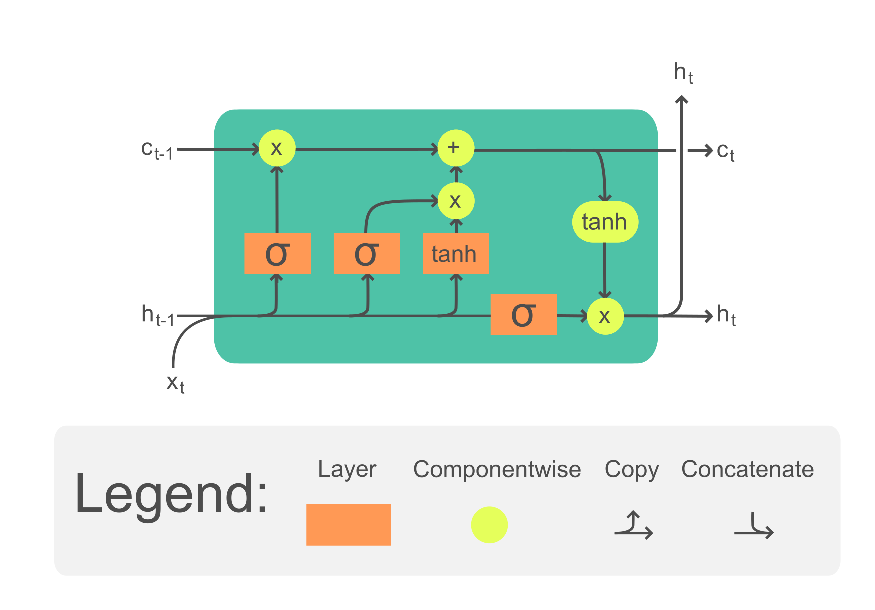
\includegraphics[width=0.7\linewidth]{figures/LSTM_Cell}
	\caption{LSTM cell,  Artist: \textcite{chevalier_english_2018}}
	\label{fig:lstmcell}
\end{figure}\todo{Do propper credit of picture}
When modeling soil temperature it is important to know the previus hours or days to predict the next timestep, for this a natural selection for a data driven model is a recurrent network. This type of network makes prediction based on previus timesteps in the data, however the longer timespan the model takse into account the less important are the erlier timesteps in the data. 

To combat this there was developed an improved model called Long-Short Term Memory model\cite{hochreiter_long_1997} that deploys a memory cell that feeds information from earlier timesteps to the late ones. To make sure that redundant information or unimportant informantion don't get feed forward there are also forgetting gates that removes some of the newly learned patterns and integrates it into the memory cell. \todo{Write more}

The most common problem in Neural networks is the vanishing gradient problem where updating the first few layers of a large network becomes exponentially more difficult since the adjustments gets smaller and smaller for each layer towards the start rather than the reverse. \gls{gl:lstm} changes this by caring information from the previous cells forward thereby allowing updating earlier cells with bigger impact than the standard approach\cite{hochreiter_long_1997}. \acrshort{ac:lstm} is part of a family of \gls{gl:rnn}'s that passes information to other cells in the same layer.



\subsection[ILSTM]{Attention aware LSTM model}\label{sec:theory:Ilstm}\todo{Consider removing if not model}

